\documentclass[../delivery_hospital_report.tex]{subfiles}
\graphicspath{ {images/}{../images/}{../../images/} }
\begin{document}

\section{Telemetria}
\subsection{Placa}

%================================ TELEMETRIA PROTÓTIPO ========================
\subsubsection{Protótipo}

\paragraph{Esquemático}

\begin{figure}[h]
\centering
    \caption{Protótipo placa de Telemetria - Esquemático principal }
    \centering % para centralizarmos a figura
    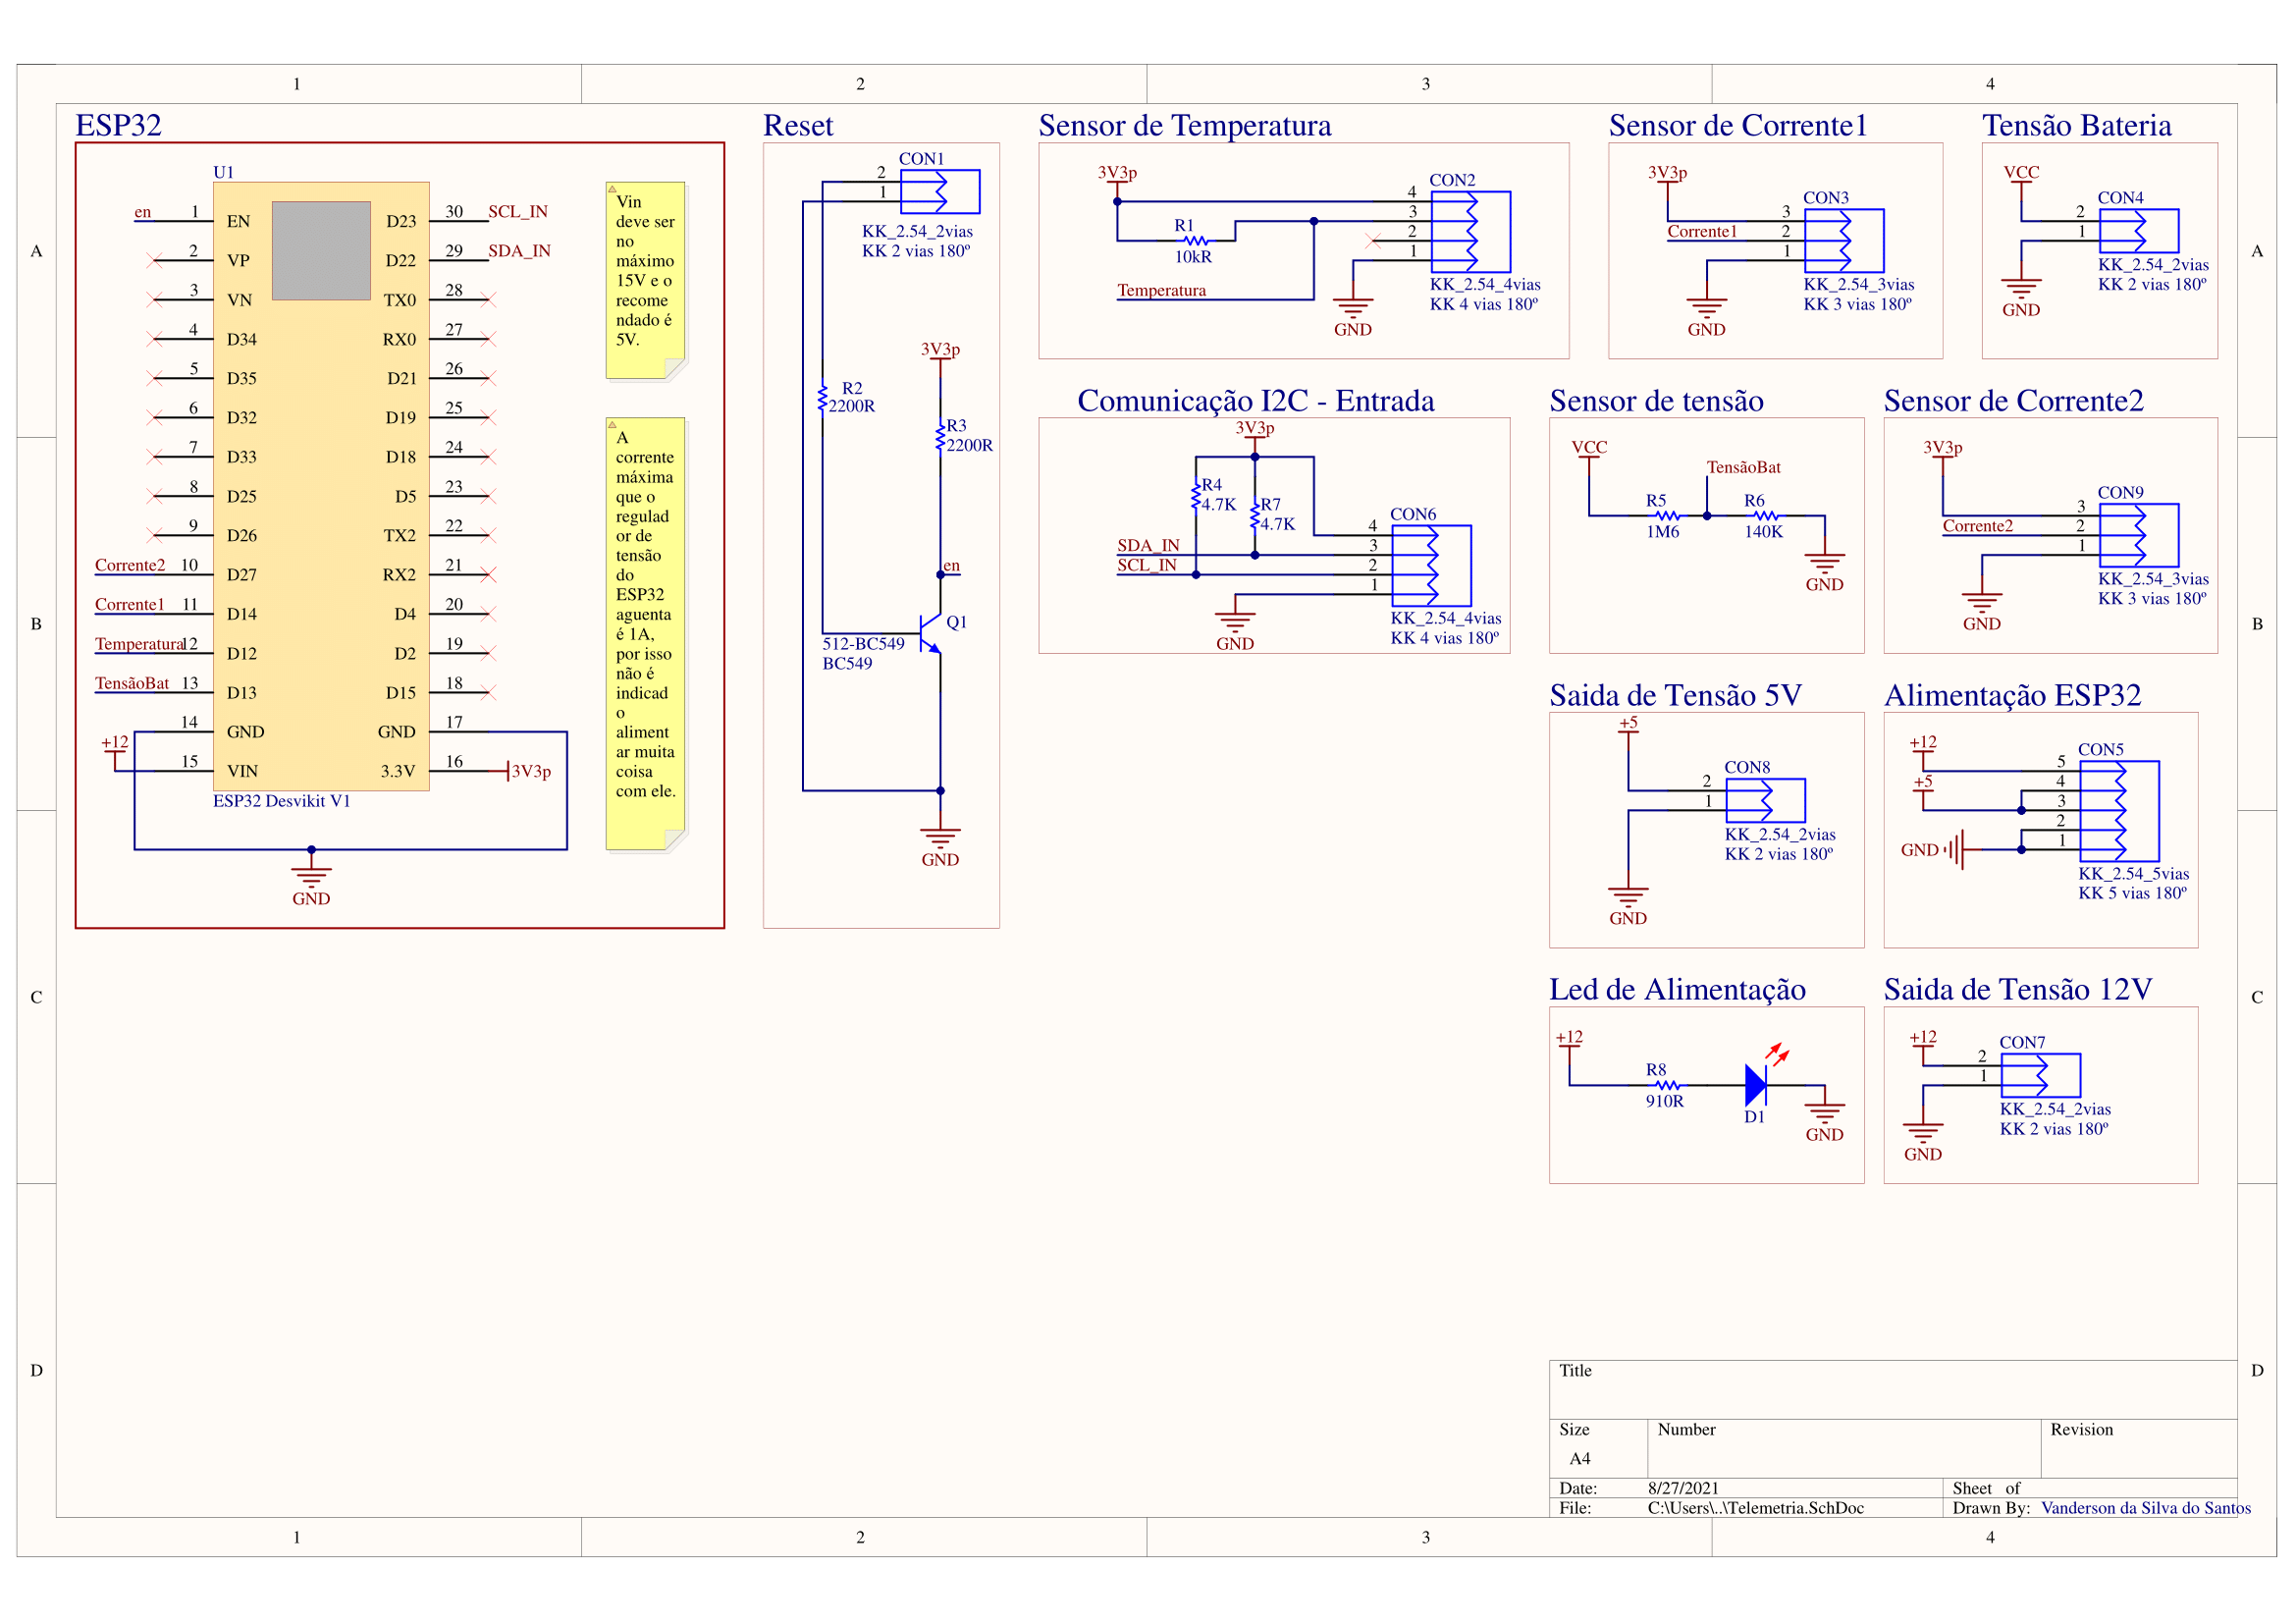
\includegraphics[width=17cm]{modulos/Telemetria-1.png}
    \caption*{Fonte: Elaborado pelo autor no software Altium Design\cite{altium21} }
    \label{Protótipo placa de ## - Esquemático principal}
\end{figure}

\begin{table}[]
\caption{Componentes Utilizados na placa de Telemetria - Protótipo}
\centering
\begin{adjustbox}{width=\columnwidth,center}
\begin{tabular}{|c|c|c|c|c|}
\hline
Component                   & Description                                    & Designator               & Footprint                   & Quantity \\ \hline
KK\_2.54\_2vias             & Conector KK 2.54mm 2   vias                    & CON1, CON4, CON7,   CON8 & KK\_2VIAS\_180º             & 4        \\ \hline
KK\_2.54\_4vias             & Conector KK 2.54mm 4   vias                    & CON2, CON6               & KK\_4vias\_180°             & 2        \\ \hline
KK\_2.54\_3vias             & Conector KK 2.54mm 3   vias                    & CON3, CON9               & KK\_3vias\_180º             & 2        \\ \hline
KK\_2.54\_5vias             & Conector KK 2.54mm 5   vias                    & CON5                     & KK\_5vias\_180°             & 1        \\ \hline
LED 5MM RED                 & LED 5MM RED                                    & D1                       & LED 5MM RED                 & 1        \\ \hline
BC549                       & TRANS NPN 30V 0.1A   TO-92                     & Q1                       & TO92                        & 1        \\ \hline
RES 470R 1/4W   CARBON FILM & RES 470R OHM 1/4W 5\%   CARBON FILM            & R1, R2, R3, R8           & RES 470R 1/4W CARBON   FILM & 4        \\ \hline
4.7K                        & RES 4.7K OHM 1/4W 5\%   CARBON FILM            & R4, R7                   & RES 4.7K 1/4W CARBON   FILM & 2        \\ \hline
1M6                         &                                                & R5                       & RESISTOR 0603               & 1        \\ \hline
140K                        &                                                & R6                       & RESISTOR 0805               & 1        \\ \hline
microcontrolador            & microcontrolador com   moculo bluethoth e wifi & U1                       & ESP32\_Desvikit\_v1         & 1        \\ \hline

\end{tabular}
\end{adjustbox}
\centering
\caption*{Fonte: Elaborado pelo autor}
\label{table:voc}
\end{table}


\paragraph{Printed Circuit board (PCB)}

\begin{figure}[!ht]
    \centering
    \begin{minipage}{0.5\textwidth}
        \centering
        \caption{Protótipo Telemetria - PCB 2D}
        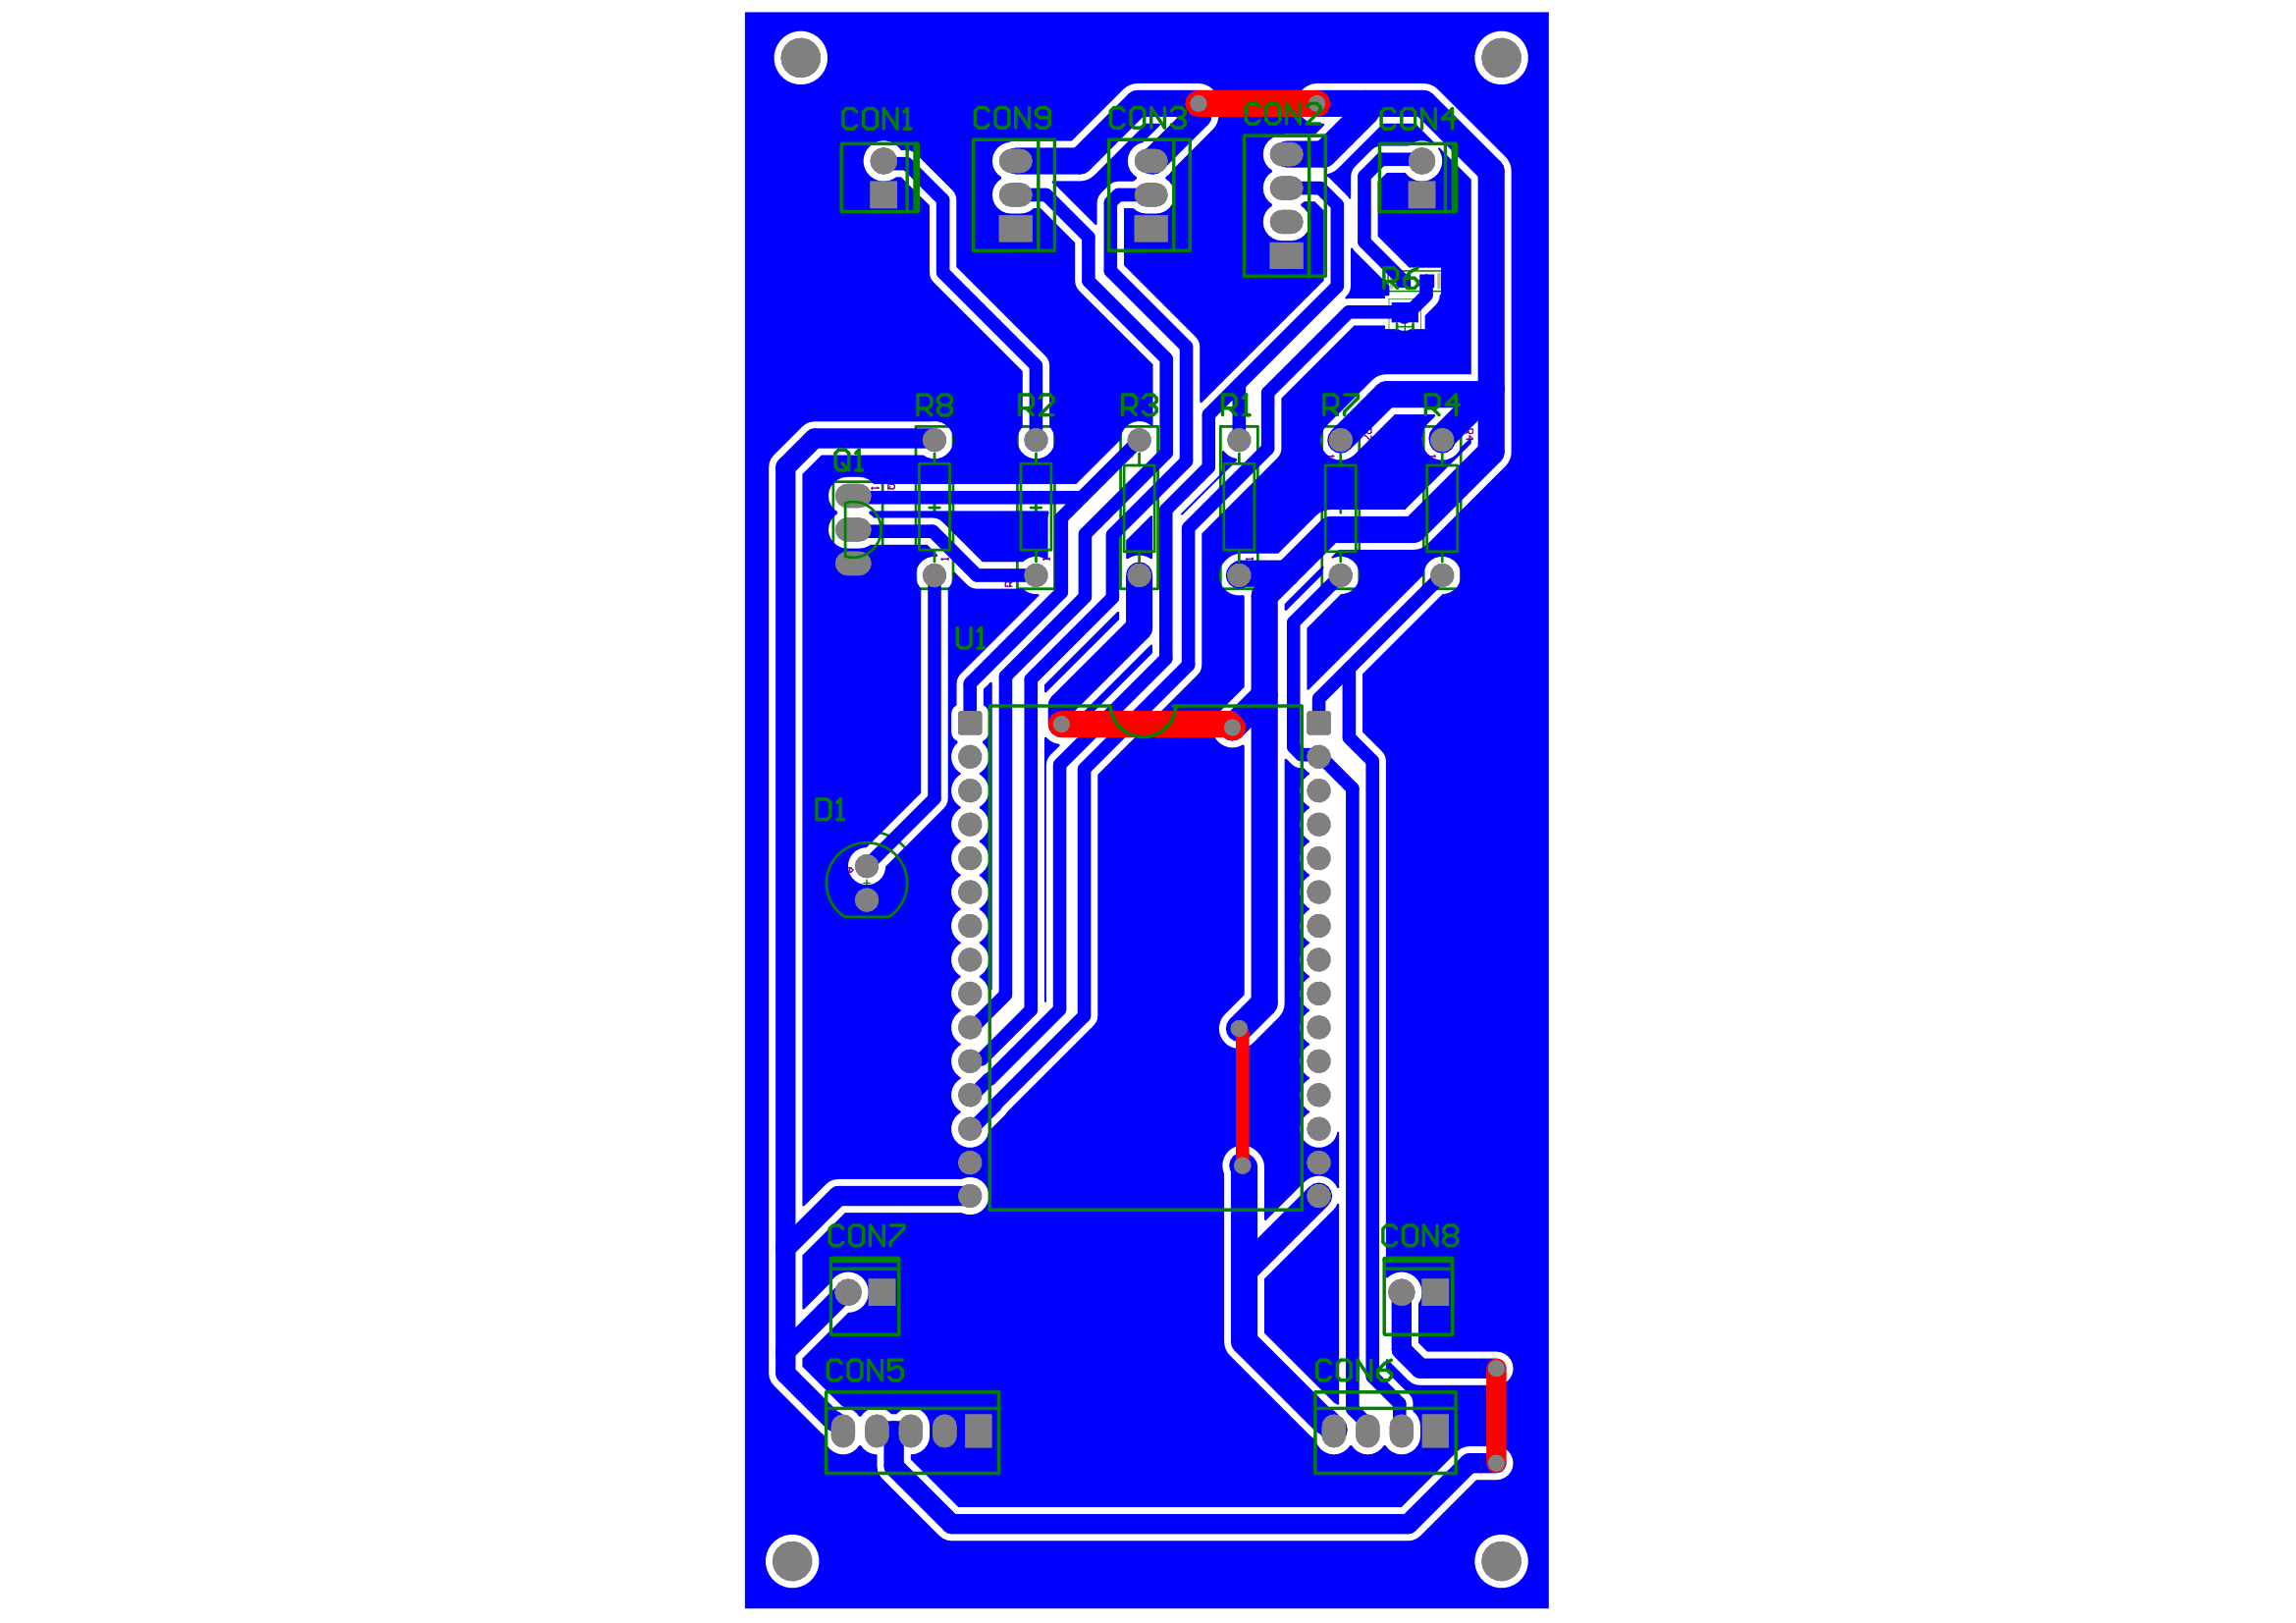
\includegraphics[width=1.03\textwidth]{modulos/Telemetria-2.png} 
        \label{fig:figura1minipg}
    \end{minipage}\hfill
    \begin{minipage}{0.5\textwidth}
        \centering
        \caption{Protótipo Telemetria - PCB 3D }
        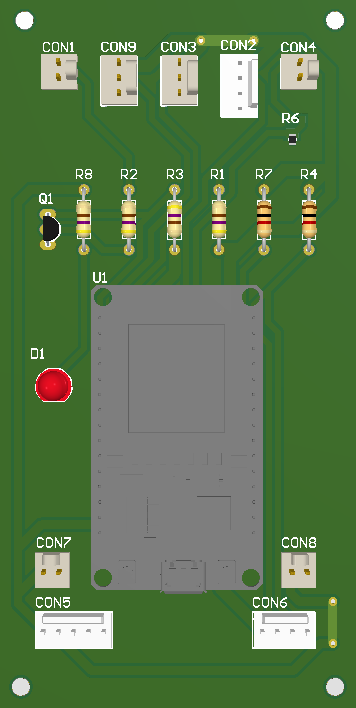
\includegraphics[width=0.4\textwidth]{modulos/Telemetria.png} 
        \label{fig:figura1minipg}
    \end{minipage}\hfill
    
    \caption*{Fonte: Elaborado pelo autor no software Altium Design\cite{altium21} }
    \label{fig:figurasminipg}
\end{figure}

\begin{figure}[!ht]
    \centering
    \begin{minipage}{0.5\textwidth}
        \centering
        \caption{Protótipo Telemetria - Trilhas}
        \includegraphics[width=0.8\textwidth]{example-image-a} 
        \label{fig:figura1minipg}
    \end{minipage}\hfill
    \begin{minipage}{0.5\textwidth}
        \centering
        \caption{Protótipo Telemetria - Completa }
        \includegraphics[width=0.8\textwidth]{example-image-a} 
        \label{fig:figura1minipg}
    \end{minipage}\hfill
    
    \caption*{Fonte: Elaborado pelo autor }
    \label{fig:figurasminipg}
\end{figure}

%================================ TELEMETRIA OFICIAL ========================
\subsubsection{Oficial}

\paragraph{Esquemático}

\begin{figure}[h]
\centering
    \caption{Placa de Telemetria - Esquemático principal }
    \centering % para centralizarmos a figura
    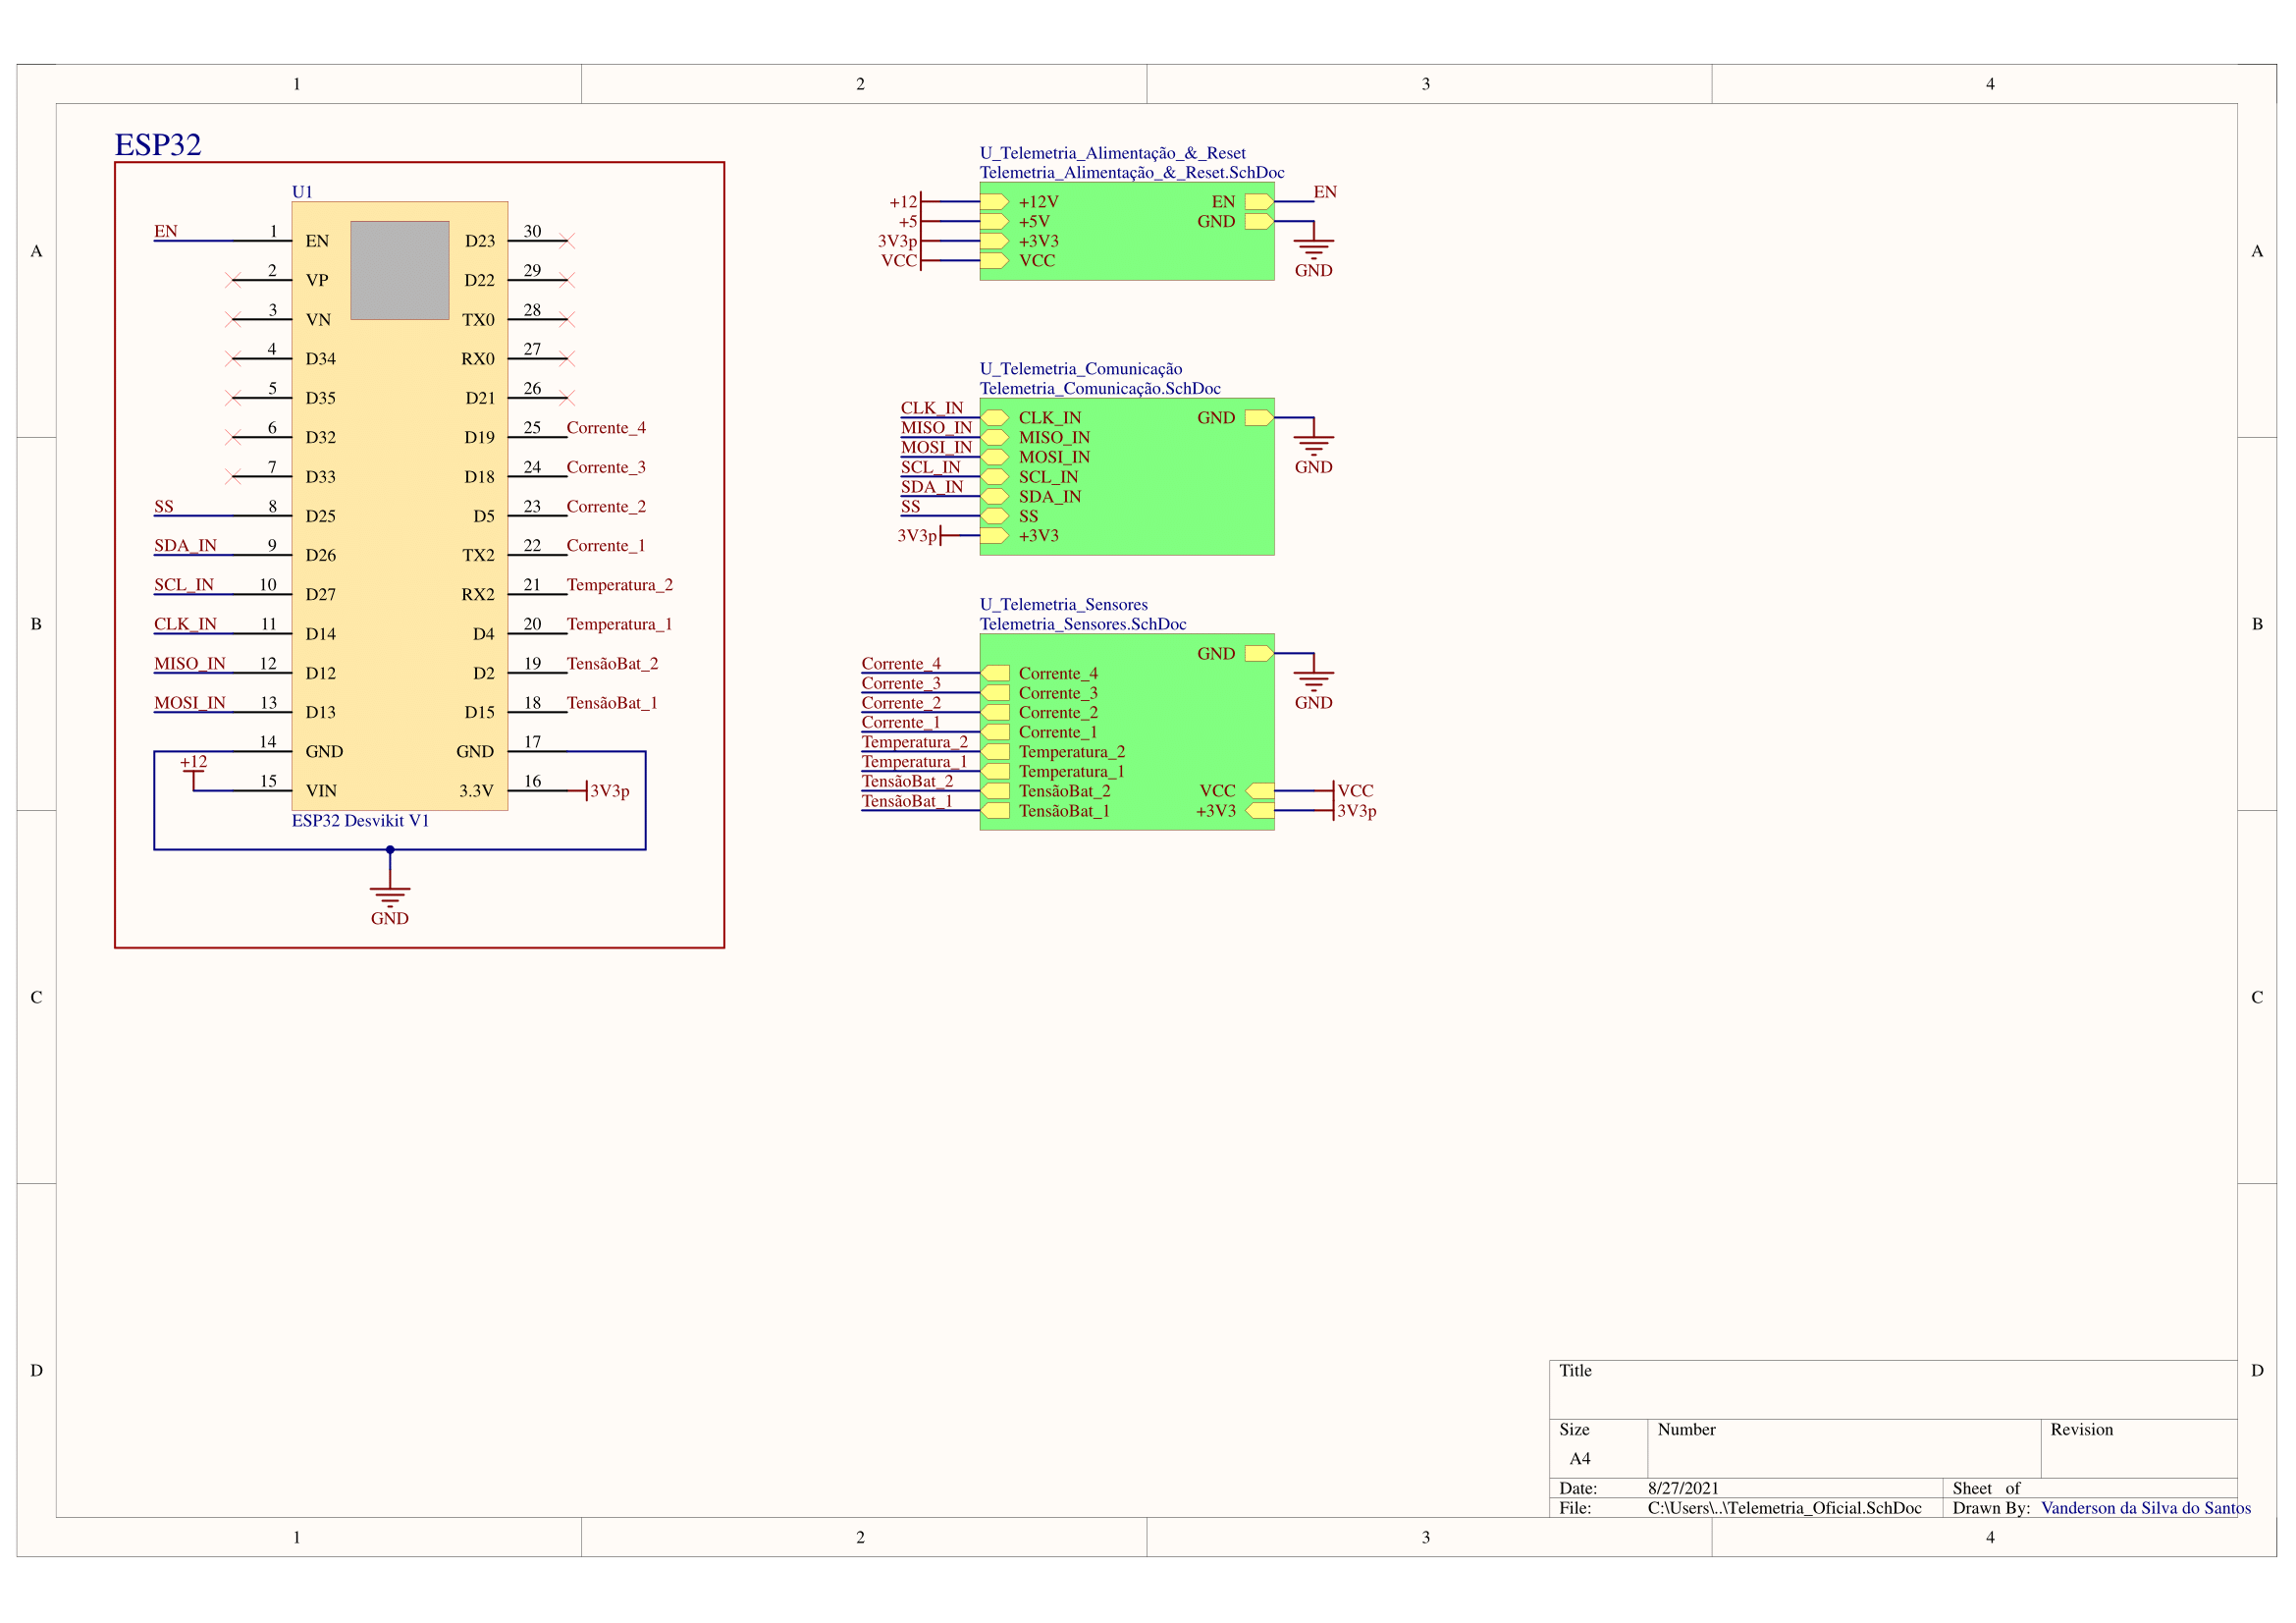
\includegraphics[width=17cm]{modulos/Telemetria_Oficial-1.png}
    \caption*{Fonte: Elaborado pelo autor no software Altium Design\cite{altium21} }
    \label{Protótipo placa de ## - Esquemático principal}
\end{figure}

\begin{table}[]
\caption{Componentes Utilizados na placa de Telemetria}
\centering
\begin{adjustbox}{width=\columnwidth,center}
\begin{tabular}{|c|c|c|c|c|}

\hline
Component        & Description                                    & Designator                  & Footprint           & Quantity \\ \hline
KK\_2.54\_2vias  & Conector KK 2.54mm 2   vias                    & CON1, CON3, CON4,   CON5    & KK\_2VIAS\_180º     & 4        \\ \hline
KK\_2.54\_6vias  & Conector KK 2.54mm 6   vias                    & CON2                        & KK\_6vias\_180°     & 1        \\ \hline
KK\_2.54\_5vias  & Conector KK 2.54mm 5   vias                    & CON6                        & KK\_5vias\_180°     & 1        \\ \hline
KK\_2.54\_4vias  & Conector KK 2.54mm 4   vias                    & CON7, CON8, CON11           & KK\_4vias\_180°     & 3        \\ \hline
KK\_2.54\_3vias  & Conector KK 2.54mm 3   vias                    & CON9, CON10, CON12,   CON13 & KK\_3vias\_180º     & 4        \\ \hline
LED 3MM RED      & LED 3MM RED                                    & D1                          & LED RED             & 1        \\ \hline
Trans BC817      & Transistor BJT NPN   BC817-25-7-F              & Q1                          & SOT96P240X110-3N    & 1        \\ \hline
680R             & Resistor                                       & R1                          & RESC3216X60N        & 1        \\ \hline
2k2              & Resistor                                       & R2, R3                      & RESC3216X60N        & 2        \\ \hline
4k7              & Resistor                                       & R4, R5                      & RESC3216X60N        & 2        \\ \hline
10k              & Resistor                                       & R6, R7                      & RESC3216X60N        & 2        \\ \hline
1M6              & 0603                                           & R8, R10                     & RESISTOR 0603       & 2        \\ \hline
140K             & 0805                                           & R9, R11                     & RESISTOR 0805       & 2        \\ \hline
microcontrolador & microcontrolador com   moculo bluethoth e wifi & U1                          & ESP32\_Desvikit\_v1 & 1        \\ \hline

\end{tabular}
\end{adjustbox}
\centering
\caption*{Fonte: Elaborado pelo autor}
\label{table:voc}
\end{table}

\paragraph{Printed Circuit board (PCB)}

\begin{figure}[!ht]
    \centering
    \begin{minipage}{0.5\textwidth}
        \centering
        \caption{Telemetria - PCB 2D}
        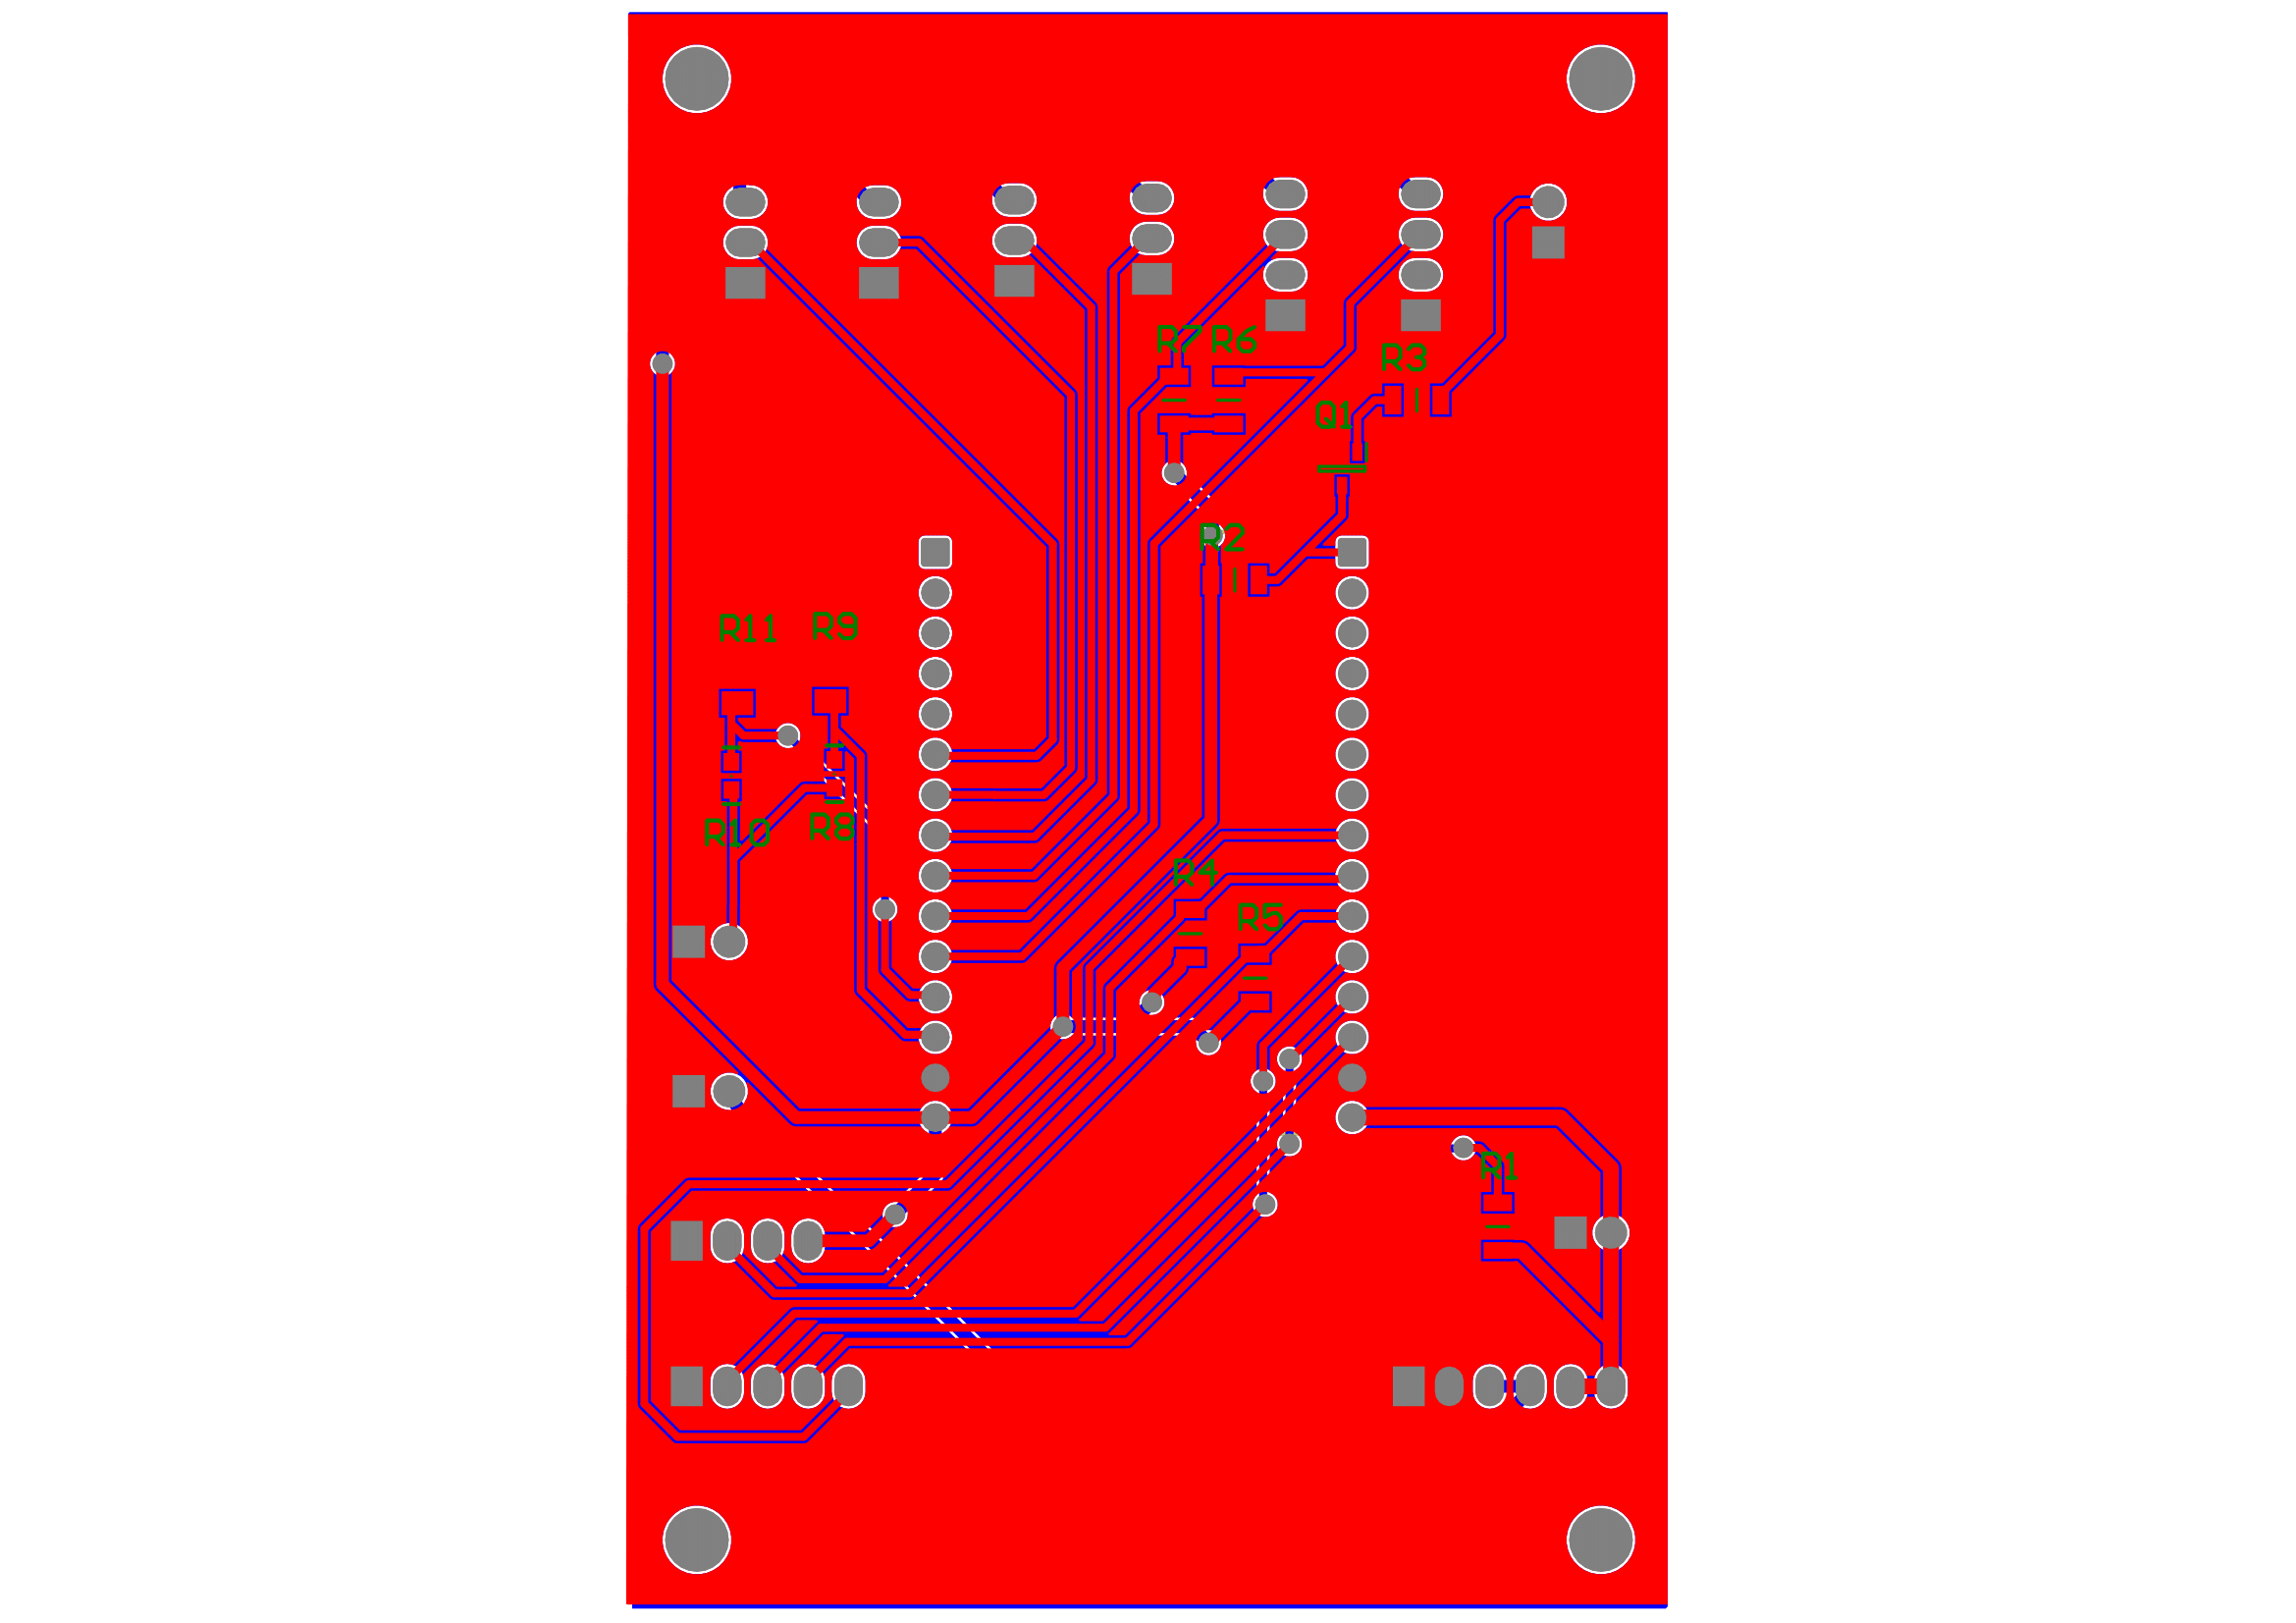
\includegraphics[width=1.03\textwidth]{modulos/Telemetria_Oficial-5.png} 
        \label{fig:figura1minipg}
    \end{minipage}\hfill
    \begin{minipage}{0.5\textwidth}
        \centering
        \caption{Telemetria - PCB 3D}
        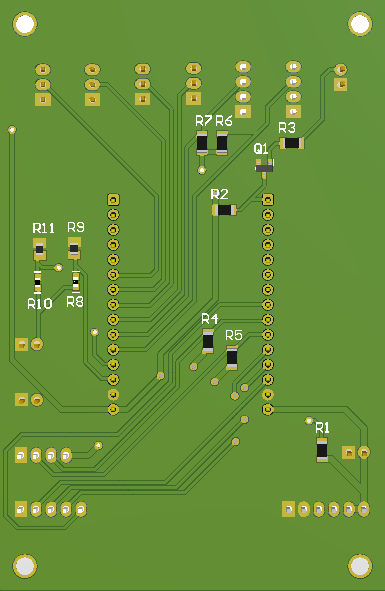
\includegraphics[width=0.4\textwidth]{modulos/Telemetria_Oficial.png} 
        \label{fig:figura1minipg}
    \end{minipage}\hfill
    
    \caption*{Fonte: Elaborado pelo autor no software Altium Design\cite{altium21} }
    \label{fig:figurasminipg}
\end{figure}

%================================ TELEMETRIA FIRMWARE ========================
\subsection{Firmware}

\end{document}